\documentclass{beamer}

\usetheme{JuanLesPins}


\usepackage[utf8]{inputenc}

\usepackage{pgfplots}
\usepackage{pgfplotstable}
\usepackage{tikz}
\usepackage{xcolor}
\usetikzlibrary{automata, arrows.meta, shapes.geometric, positioning}

\usepackage{minted}
\usepackage{todonotes}
\usepackage[normalem]{ulem}
\usepackage[export]{adjustbox}



% \newtheorem{theorem}{Theorem}[chapter]
% \newtheorem{corollary}{Corollary}[theorem]
% \newtheorem{lemma}[theorem]{Lemma}
% \newtheorem{proposition}[theorem]{Proposition}
% \theoremstyle{definition}
% \newtheorem{example}[theorem]{Example}
% \newtheorem{definition}[theorem]{Definition}



\newcommand{\ZZ}{\mathbb{Z} \times \mathbb{Z}}
\newcommand{\nequiv}{\not\equiv}
\newcommand{\nequivp}{\nequiv_{\Psi,\T}}
\newcommand{\equivp}{\equiv_{\Psi,\T}}
% \renewcommand{\labelenumii}{\arabic{enumii}.}
\newcommand{\join}{\sqcup}
\newcommand{\meet}{\sqcap}
\newcommand{\widen}{\nabla}
\newcommand{\narrow}{\Delta}
\newcommand{\sem}[1]{\llbracket#1\rrbracket}
\newcommand{\Z}{\mathbb{Z}}
\renewcommand{\L}{\mathcal{L}}
\newcommand{\T}{\mathcal{T}}
\newcommand{\Set}{\mathcal{S}}
\newcommand{\oT}{{\overline{\mathcal{T}}}}
\newcommand{\F}{\mathcal{F}}
\newcommand{\A}{\mathcal{A}}
\newcommand{\X}{\mathcal{X}}
\newcommand{\V}{\mathcal{V}}
\newcommand{\malloc}{\textsf{malloc}}
\newcommand{\nf}{\textsf{nf}}
\newcommand{\restr}[2]{\left.\kern-\nulldelimiterspace#1\vphantom{|}\right|_{#2}}
\newcommand{\otau}{\overline{\tau}}
\newcommand{\angl}[1]{\langle#1\rangle}
% \newcommand{\widen}{\mathop{{\sqcup}\hspace*{-0.6em}\raisebox{.4ex}{\setlength{\unitlength}{1em}\line(1,0){.53}}}}
% \newcommand{\narrow}{\mathop{{\sqcap}\hspace*{-0.6em}\raisebox{.9ex}{\setlength{\unitlength}{1em}\line(1,0){.50}}}}
\newcommand{\ignore}[1]{}
\newcommand{\cpo}{\textsf{C-2PO}}
\newcommand{\goblint}{\textsc{Goblint}}
\newcommand{\find}[1]{\textsf{find}(#1)}
\newcommand{\union}[3]{\textsf{union}(#1, #2, #3)}
\newcommand{\closure}[4]{\textsf{closure}(#4, #1 = #2 + #3)}
\newcommand{\ext}[2]{\textsf{ext}\,{#1}\,{#2}}
\newcommand{\enter}{\textsf{enter}}
\newcommand{\combine}{\textsf{combine}}
\newcommand{\base}{\emph{base}}
\newcommand{\vareq}{\emph{var\_eq}}
\newcommand{\cpou}{$c$-$2po_1$}
\newcommand{\cpod}{$c$-$2po_2$}
\newcommand{\cpot}{$c$-$2po_3$}
\newcommand{\cpoq}{$c$-$2po_4$}


% Define TUM corporate design colors
% Taken from http://portal.mytum.de/corporatedesign/index_print/vorlagen/index_farben
\definecolor{TUMBlue}{HTML}{0065BD}
\definecolor{TUMSecondaryBlue}{HTML}{005293}
\definecolor{TUMSecondaryBlue2}{HTML}{003359}
\definecolor{TUMBlack}{HTML}{000000}
\definecolor{TUMWhite}{HTML}{FFFFFF}
\definecolor{TUMDarkGray}{HTML}{333333}
\definecolor{TUMGray}{HTML}{808080}
\definecolor{TUMLightGray}{HTML}{CCCCC6}
\definecolor{TUMAccentGray}{HTML}{DAD7CB}
\definecolor{TUMAccentOrange}{HTML}{E37222}
\definecolor{TUMAccentGreen}{HTML}{A2AD00}
\definecolor{TUMAccentLightBlue}{HTML}{98C6EA}
\definecolor{TUMAccentBlue}{HTML}{64A0C8}



\title[Weakly-Relational Pointer Analysis]{A Weakly-Relational Pointer Analysis for the Goblint Abstract Interpreter}
\author{Rebecca Ghidini}
\date{\today}

\begin{document}
\maketitle

\section{Introduction}
\frame{\tableofcontents[currentsection]}

\begin{frame}{Motivation}
    \begin{itemize}
        \item Pointer analysis
        \item \emph{Weakly} relational: relations between pairs of pointer expressions, e.g.,
              \[
                  \&x = 4 + \&y
              \]
    \end{itemize}
\end{frame}

\begin{frame}[containsverbatim]{Example}
    %(etwas was goblint noch nicht konnte auch nicht mit var eq
    %-> running example)
    \begin{minipage}{0.49\textwidth}

        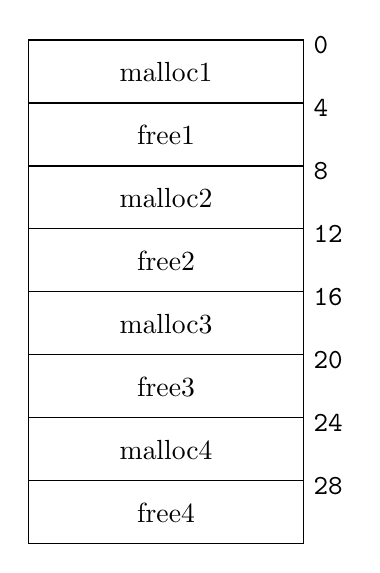
\begin{tikzpicture}

            % Settings
            \def\blockheight{0.8}
            \def\blockwidth{3.5}

            % Memory blocks and addresses
            \foreach \i/\label in {0/malloc1, 1/free1, 2/malloc2, 3/free2, 4/malloc3, 5/free3, 6/malloc4, 7/free4} {
                    % Draw memory block
                    \draw (0, -\i*\blockheight) rectangle (\blockwidth, -\i*\blockheight - \blockheight);
                    % Label the memory block
                    \node at (\blockwidth/2, -\i*\blockheight - \blockheight/2) {\label};
                    % Print address to the right
                    \node[above right=0.1cm and 0cm] at (\blockwidth, -\i*\blockheight - \blockheight/2) {\texttt{\the\numexpr 4*\i \relax}};
                }
        \end{tikzpicture}
    \end{minipage}
    \begin{minipage}{0.49\textwidth}

        \begin{minted}{C}
...
(*malloc)(p);
...
(*free)(p);
...
\end{minted}
        $\rightarrow$ $free = 4 + malloc$?
    \end{minipage}
\end{frame}

\begin{frame}{Why are disequalities important}
    TODO
    not the same memory block etc
\end{frame}

\section{Abstract Domain}
\frame{\tableofcontents[currentsection]}

\begin{frame}{Abstract Domain}
    \begin{itemize}
        \item Set of terms $\T$
              $\{A, *A, \&x, x, \&y, y, *(1+y)\}$
        \item Conjunction of equalities and disequalities:
              \begin{itemize}
                  \item Quantitative equalities
                        \[
                            (A = 1 + y) \land (\&x = \&y)
                        \]
                  \item Quantitative disequalities
                        \[
                            (x \neq 4 - y)
                        \]
                  \item Block disequalities
                        \[
                            (bl(y) \neq bl(A))
                        \]
              \end{itemize}
    \end{itemize}
\end{frame}

\begin{frame}{Quantitative Finite Automaton (QFA)}
    \todo[inline]{How to add equalities?}
    \[
        \T=\{A, *(1 + A), \&x, x, \&y, y, *y\}
    \]
    \[
        (y = 1 + A) \land (\&x = \&y)
    \]
    \centering
    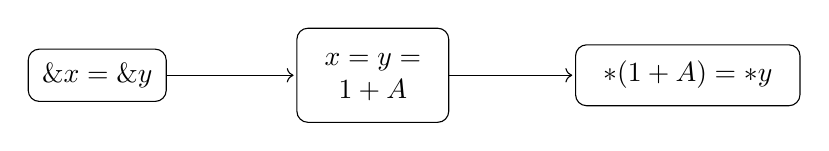
\begin{tikzpicture}[shorten >=1pt, node distance=5cm, on grid, auto, state/.style={rectangle, rounded corners, draw, inner sep=5pt, align=center}]

        \node[state] (y) {$\&x =\&y$};

        \node[state, right=3.5cm of y] (AB) {$\begin{array}{c}
                    x = y = \\
                    1 + A
                \end{array}$};

        \node[state, right=4cm of AB] (ABs) {$\begin{array}{c}
                    *(1+A) = *y
                \end{array}$};

        \path[->]
        (y) edge[] (AB)
        (AB) edge[] (ABs);


    \end{tikzpicture}
\end{frame}

\begin{frame}{QFA: Insert Terms}
    \[
        \T=\{A, *(1 + A), \&x, x, \&y, y, *y, \textcolor{TUMAccentOrange}{*x}\}
    \]
    \[
        (y = 1 + A) \land (\&x = \&y)
    \]
    \centering
    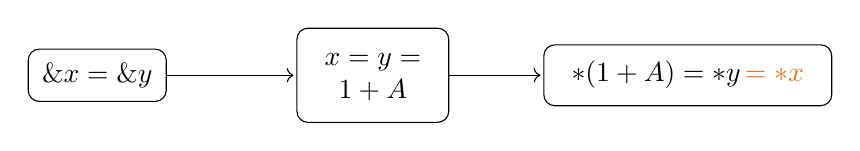
\begin{tikzpicture}[shorten >=1pt, node distance=5cm, on grid, auto, state/.style={rectangle, rounded corners, draw, inner sep=5pt, align=center}]

        \node[state] (y) {$\&x =\&y$};

        \node[state, right=3.5cm of y] (AB) {$\begin{array}{c}
                    x = y = \\
                    1 + A
                \end{array}$};

        \node[state, right=4cm of AB] (ABs) {$\begin{array}{c}
                    *(1+A) = *y \textcolor{TUMAccentOrange}{\,= *x}
                \end{array}$};

        \path[->]
        (y) edge[] (AB)
        (AB) edge[] (ABs);


    \end{tikzpicture}


\end{frame}

\begin{frame}{restriction}
    TODO
\end{frame}

\begin{frame}[containsverbatim]{Block Disequalities}
    \begin{itemize}
        \item Two terms do not belong to the same C block
        \item For all variables $x$ and $y$:
              \[
                  bl(\&x) \neq bl(\&y)
              \]
        \item
              \begin{minted}{C}
int *x = malloc();
int *y = malloc();
\end{minted}

              \[
                  bl(x) \neq bl(y)
              \]

    \end{itemize}
\end{frame}

\begin{frame}[containsverbatim]{Quantitative Disequalities}
    \begin{itemize}
        \item Deriving from block disequalities: If $bl(t_1) \neq bl(t_2)$
              \[
                  t_1\neq z+ t_2 \quad\quad \text{for each $z \in \Z$}
              \]
        \item Deriving from equalities: If $t_1 = z + t_2$,
              \[
                  t_1\neq z' + t_2 \quad\quad \text{for each $z' \neq z$}
              \]

        \item Deriving from guards:
              \begin{minted}{C}
if(*x != 4 + y){...}
\end{minted}
        \item Deriving from other disequalities: If $*(z_1 + t_1) \neq *(z_2 + t_2)$,
              \[ t_1 \neq (z_2 - z_1) + t_2
              \]
    \end{itemize}
\end{frame}

\section{Partial Order}

\begin{frame}{Equality}
    \todo[inline]{partial order}
    \begin{Definition}
        Eine Definition
    \end{Definition}
\end{frame}

\section{Meet}
\begin{frame}{Meet}
    \begin{itemize}

        \item Equivalent to conjunction $\land$
        \item Update parition and QFA
        \item Add block/quantitative disequalities
        \item Closure of disequalities

    \end{itemize}
\end{frame}

\section{Join}
\begin{frame}{Join}
    \[
        \T = \{
        \&x,x,*x, {*}{*}x
        \}
    \]
    \begin{minipage}{0.4\textwidth}
        \centering
        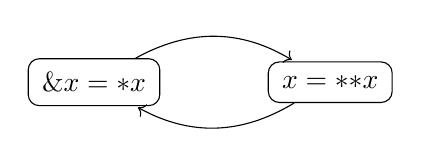
\begin{tikzpicture}[shorten >=1pt, node distance=3cm, on grid, auto, state/.style={rectangle, rounded corners, draw, inner sep=5pt, align=center}]

            \node[state, initial text={}] (Q1) {$\&x= *x$};
            \node[state, right=of Q1] (Q2) {$x= {*}{*}x$};

            \path[->]
            (Q1) edge[bend left, above] (Q2)
            (Q2) edge[bend left, below] (Q1);

        \end{tikzpicture}

        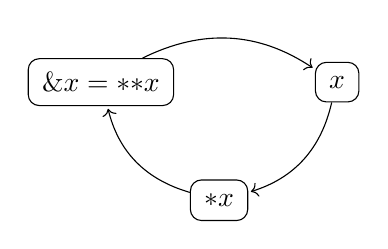
\begin{tikzpicture}[shorten >=1pt, node distance=3cm, on grid, auto, state/.style={rectangle, rounded corners, draw, inner sep=5pt, align=center}]

            \node[state, initial text={}] (Q1) {$\&x= {*}{*}x$};
            \node[state, right=of Q1] (Q2) {$x$};
            \node[state, below right=1.5cm and 1.5cm of Q1] (Q3) {$*x$};


            \path[->]
            (Q1) edge[bend left] (Q2)
            (Q2) edge[bend left] (Q3)
            (Q3) edge[bend left] (Q1);

        \end{tikzpicture}
    \end{minipage}
    \begin{tikzpicture}[overlay]
        \draw[->, thick] (0, 0) -- (1, 0);
    \end{tikzpicture}
    \hfill%
    \begin{minipage}{0.49\textwidth}

        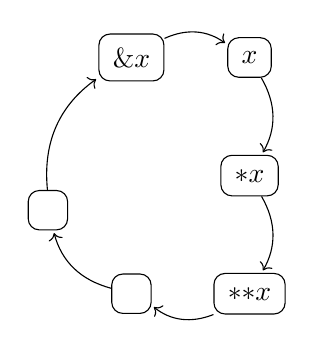
\begin{tikzpicture}[shorten >=1pt, node distance=1.5cm, on grid, auto, state/.style={rectangle, rounded corners, draw, inner sep=5pt, align=center, minimum size=0.5cm}]

            \node[state, initial text=] (Q1) {$\&x$};
            \node[state, right= 1.5cm of Q1] (Q2) {$x$};
            \node[state, below=of Q2] (Q3) {$*x$};
            \node[state, below=of Q3] (Q4) {${*}{*}x$};
            \node[state, left=of Q4] (Q5) {};
            \node[state, above left=of Q5] (Q6) {};




            \path[->]
            (Q1) edge[bend left] (Q2)
            (Q2) edge[bend left] (Q3)
            (Q3) edge[bend left] (Q4)
            (Q4) edge[bend left] (Q5)
            (Q5) edge[bend left] (Q6)
            (Q6) edge[bend left] (Q1)
            ;

        \end{tikzpicture}
    \end{minipage}
\end{frame}


\begin{frame}{Join}
    \begin{itemize}
        \item Add a term for each empty state in the automaton
    \end{itemize}
    \[
        \T = \{
        \&x,x,*x, {*}{*}x,\textcolor{TUMAccentOrange}{{*}{*}{*}x,{*}{*}{*}{*}x}
        \}
    \]

    \centering
    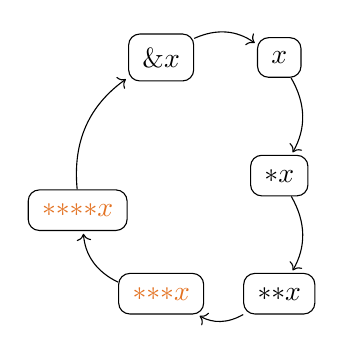
\begin{tikzpicture}[shorten >=1pt, node distance=1.5cm, on grid, auto, state/.style={rectangle, rounded corners, draw, inner sep=5pt, align=center, minimum size=0.5cm}]

        \node[state, initial text=] (Q1) {$\&x$};
        \node[state, right= 1.5cm of Q1] (Q2) {$x$};
        \node[state, below=of Q2] (Q3) {$*x$};
        \node[state, below=of Q3] (Q4) {${*}{*}x$};
        \node[state, left=of Q4] (Q5) {$\textcolor{TUMAccentOrange}{{*}{*}{*}x}$};
        \node[state, above left=of Q5] (Q6) {$\textcolor{TUMAccentOrange}{{*}{*}{*}{*}x}$};
        \path[->]
        (Q1) edge[bend left] (Q2)
        (Q2) edge[bend left] (Q3)
        (Q3) edge[bend left] (Q4)
        (Q4) edge[bend left] (Q5)
        (Q5) edge[bend left] (Q6)
        (Q6) edge[bend left] (Q1)
        ;

    \end{tikzpicture}
\end{frame}

\section{Widening and Narrowing}
\begin{frame}{Widening}
    \begin{itemize}
        \item Infinite strictly ascending chain:
    \end{itemize}
    \[
        \Psi_n \equiv (*^{2^n} \&x = \&x)\hspace{6pt} (n\geq 0).
    \]
    \begin{itemize}
        \item Limit the terms of the result to the set of terms of the first element
    \end{itemize}
    \[\Psi_1 \widen \Psi_2 = \restr{(\Psi_1 \join \Psi_2)}{\T_1}.\]
\end{frame}

\begin{frame}{Narrowing}
    \begin{itemize}
        \item Infinite strictly descending chains:
    \end{itemize}
    \[
        \Phi_n \equiv\bigwedge_{i=1}^n (\&y = *(i+\&x))\qquad(n\geq 0)
    \]
    \[
        \Psi_n \equiv (y\neq n+\&x)\qquad(n\geq 0)
    \]
    \begin{itemize}
        \item Limit the terms of the result and the possible offsets
              appearing in disequalities -> to what?
    \end{itemize}

\end{frame}

\section{Assignment}

\begin{frame}{Assignment}
    \[
        t_1\,{:=}\,?
    \]
    \begin{itemize}
        \item Forget all terms that may be modfied $\rightarrow$ terms that have the same address
        \item If $t_1 = A$ or $t_1 = \&x$: remove terms that have $t_1$ as subterm
        \item If $t_1 = *(z + t)$: keep only terms $*(z' + v)$ where $t \neq (z' - z) + v$
              \begin{itemize}
                  \item $t = z_1 + v$ and $z_1 \neq (z' - z)$ and they do not overlap
                  \item $t \neq (z' - z) + v$ or $bl(t) \neq bl(v)$
                  \item use non-relational analysis: possible values of $t$ and $(z' - z) + v$ do not intersect
              \end{itemize}
    \end{itemize}
\end{frame}

\begin{frame}{Assignment}
    \[
        t_1\,{:=}\,z + t
    \]
    \begin{itemize}
       \item Fresh auxiliary $A$
       \item Add equality $A = z + t$
       \item Remove terms modified by an assignment to $t_1$
       \item Add equality $t_1 = A$
       \item Remove $A$
    \end{itemize}
\end{frame}

\begin{frame}{Assignment}
    \[
        t_1\,{:=}\,\malloc
    \]
    \begin{itemize}
       \item For each $t \in \T$, add:
       \[
       bl(t) \neq bl(t_1)
       \]
    \end{itemize}
\end{frame}

\section{Evaluation}
\frame{\tableofcontents[currentsection]}

\begin{frame}{Precision}
\end{frame}
\begin{frame}{Litmus Tests}
    \begin{tikzpicture}
        \begin{axis}[
                ybar,
                symbolic x coords={\base, \vareq, \cpo},
                xtick=data,
                ymin=0, ymax=109,
                bar width=1cm,
                ylabel={Number of Proven Assertions},
                xlabel={Analyses},
                nodes near coords,
                nodes near coords align={vertical},
            ]
            \addplot coordinates {(\base, 17) (\vareq, 23) (\cpo, 109)};
        \end{axis}
    \end{tikzpicture}

\end{frame}

\begin{frame}{Coreutils Tests}
    \begin{tikzpicture}
        \begin{axis}[
                ybar,
                symbolic x coords={\base, \vareq, \cpo},
                xtick=data,
                ymin=0, ymax=19488,
                bar width=1cm,
                ylabel={Number of Proven Assertions},
                xlabel={Analyses},
                nodes near coords,
                nodes near coords align={vertical},
            ]
            \addplot coordinates {(\base, 4636) (\vareq, 8188) (\cpo, 19488)};
        \end{axis}
    \end{tikzpicture}

\end{frame}

\begin{frame}{Performance}

\end{frame}

\begin{frame}{SV-Comp Results}
    \includegraphics[scale=0.3]{images/base-vs-cpo4.png}
\end{frame}

\section{Conclusion}
\frame{\tableofcontents[currentsection]}

\begin{frame}{Conclusion}
    was haben wir gelernt, ist sie geeignet, was sind die vorteile
    man kann auch unsere analyse benutzen um zu wissen, ob sachen bei einem assignment überschrieben werden, so wie wir die non-relational pointer analyse benutzen
\end{frame}

\appendix

\begin{frame}[allowframebreaks]
    \frametitle{References}
    \bibliographystyle{amsalpha}
    \bibliography{main.bib}
\end{frame}

\begin{frame}{Representation of structs and arrays}
    \begin{Definition}
        Eine Definition
    \end{Definition}
\end{frame}



\begin{frame}{Interprocedural?}
    \begin{Definition}
        Eine Definition
    \end{Definition}
\end{frame}


\begin{frame}{Overlapping values}

    {
        \centering

        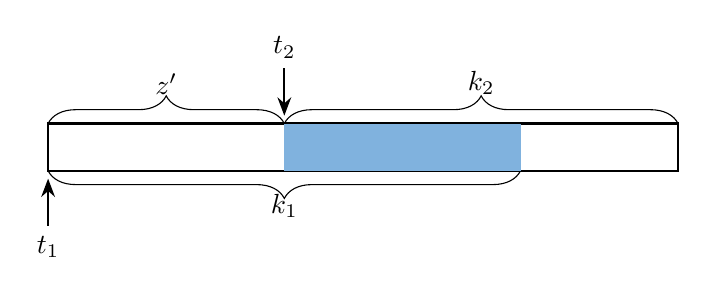
\begin{tikzpicture}[
                memory/.style={draw, thick, minimum height=0.6cm},
                pointer/.style={-Stealth, thick},
                bracket/.style={decorate,decoration={brace, amplitude=10pt, mirror}},
                bracketabove/.style={decorate,decoration={brace, amplitude=10pt}}
            ]

            \draw[memory] (0,0) rectangle (8,0.6);

            \draw[pointer] (3, 1.3) node[above] {$t_2$} -- (3, 0.7);
            \draw[pointer] (0, -0.7) node[below] {$t_1$} -- (0, -0.1);

            \draw[bracketabove] (3, 0.6) -- node[above=7pt] {$k_2$} (8, 0.6);
            \draw[bracketabove] (0, 0.6) -- node[above=7pt] {$z'$} (3, 0.6);
            \draw[bracket] (0, 0) -- node[below=5pt] {$k_1$} (6, 0);

            \draw[dashed] (3, 0) -- (3, 0.6);
            \draw[dashed] (6, 0) -- (6, 0.6);

            \fill[TUMBlue!50] (3,0) rectangle (6,0.6); % overlap

        \end{tikzpicture}
    }
    \begin{itemize}
        \item $t_2 \equiv_{k} z' + t_1$.
        \item There is an overlap if $z' < k_1$.
    \end{itemize}

\end{frame}

\end{document}
